\begin{figure*}[t]
\centering
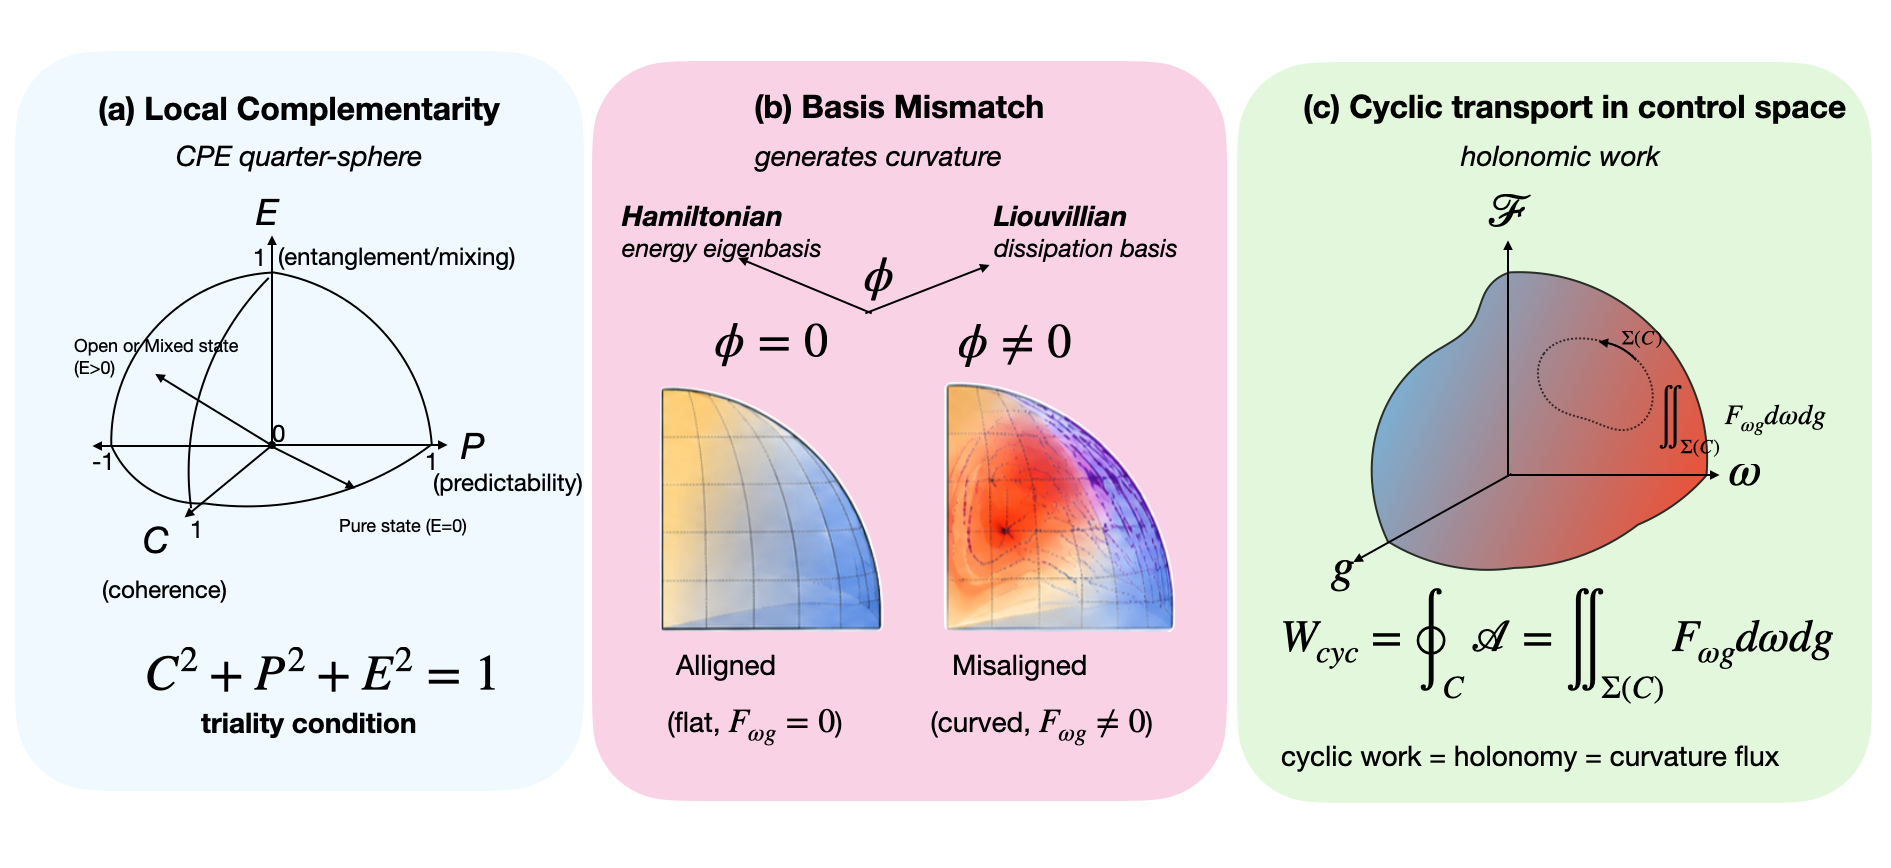
\includegraphics[width=\textwidth]{Figures/CPE_Fig0.png}
\caption{
\textbf{Complementarity and the triality manifold for open quantum systems.}
(a) The complementarity variables coherence $C$,
predictability $P$, and openness $E$ provide a natural
coordinate system for the reduced steady-state manifold of
a driven qubit. These variables satisfy the normalized
triality relation
$C^{2}+P^{2}+E^{2}=1$,
so that every physically admissible reduced state occupies
a point on the quarter sphere. Coherence measures the
off-diagonal quantum superposition within the pointer-basis
plane, predictability measures the population imbalance,
and openness quantifies the contraction of the Bloch sphere
resulting from environmental mixing.
(b) Schematic illustration of the competition between
coherent Hamiltonian evolution and environmentally selected
pointer states. When the Hamiltonian and pointer bases are
aligned, the stationary state reduces to the Gibbs manifold
and the response is integrable. Misalignment between these
structures produces genuinely nonequilibrium steady states
whose response cannot, in general, be derived from a global
thermodynamic potential.
(c) Conceptual representation of quasistatic transport over
the control manifold. Cyclic evolution generates a geometric
response that depends upon the path taken through parameter
space rather than only the initial and final states. The
formal relationship between the local response tensor, the
antisymmetric response field, and the resulting cyclic work
is developed in the following sections.
Throughout this review, the triality manifold serves as the
canonical state-space representation for open quantum
systems. The complementarity variables $(C,P,E)$ specify
the local steady state, while subsequent figures paint
response fields onto this manifold to illustrate the
relationship between complementarity, nonequilibrium
response, geometric transport, and observational
reconstruction.
}
\label{fig:CPE}
\end{figure*}